\section{Vježba 4: SURF}

\subsection{Opis vježbe}
Izraditi 2D model nekog objekta na temelju slike tog objekta snimljenog
kamerom. Razmatrani model predstavlja skup 2D točaka detektiranih
SURF-metodom kojima su pridruženi lokalni deskriptori.  Potrebno je
raspoznati objekt na drugoj slici koja je također snimljena kamerom, ali
iz drugog položaja.  
\\
\begin{lstlisting}[language=bash,caption={Pokretanje programa iz
    komandne linije}]
$ ./feature_matching ../images/sm-object.jpg ../images/sm-scene.jpg 
\end{lstlisting}

\subsection{Objašnjenje programa}

\subsubsection{Kontrola programa}

Prilikom pokretanja programa iz komandne linije potrebno je 
predati programu putanju do slike objekta (argv[1]) i putanju do slike
scene (argv[2]). 
\\

\begin{lstlisting}[language=C,caption={Kontrola programa tipkovnicom}]
while (1){
    char c = waitKey(10);
    switch(c) {
            case 's':
                surfFlannMatcher ();
                break;
\end{lstlisting}


\subsubsection{SURF}

\begin{lstlisting}[language=C,caption={Racunanje parametra ro i theta}]
\end{lstlisting}

\begin{figure}[h]
\centering
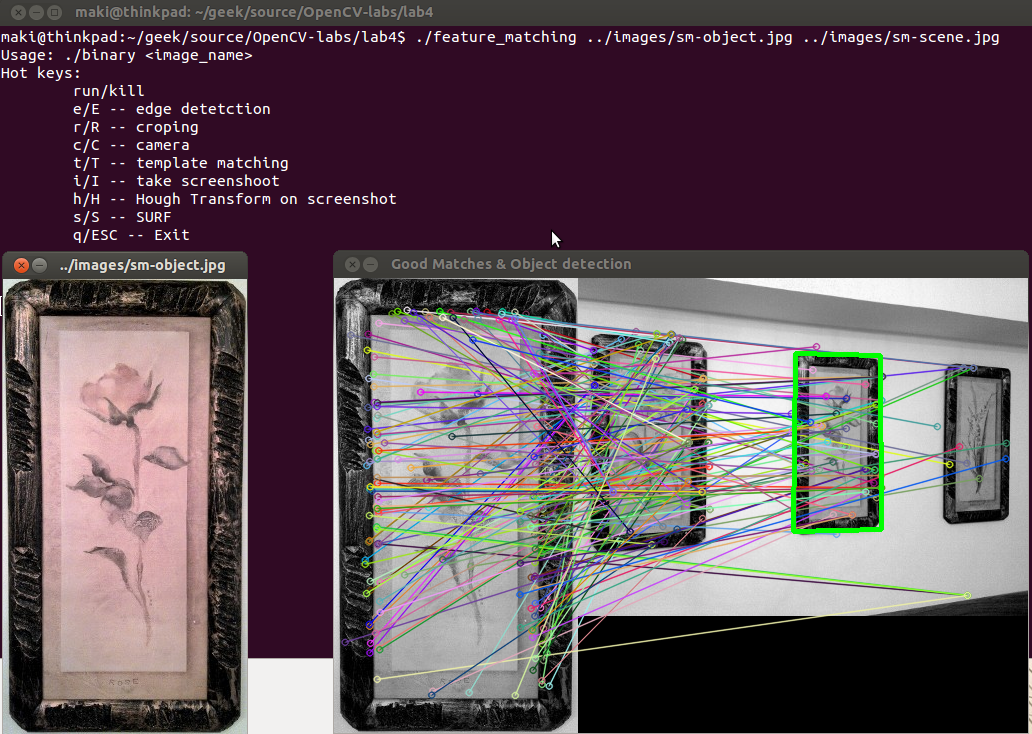
\includegraphics[scale=0.42]{images/lab4-surf-01.png}
\caption{SURF - pronalazak objekta u sceni}
\label{fig:lab4-surf-01}
\end{figure}

\newpage
\subsection{Zaključak}
